\section{Experimental results}

As we have defined earlier, a decoding failure is an instance where, on input $(H,s)$, where $s$ is of the form $s=He^T$, the syndrome decoder output $e'$ is such that $He'^T \ne s$ or $e' \ne e$.  The experiment was also designed to record any decoding instances where $He'^T=s$ and $e'\ne e$, but none were discovered. For the security level $\lambda = 20$, we manage to reproduce the error floor region as predicted in \cite{Richardson03}.

\begin{figure}[htbp]
  \begin{center}
    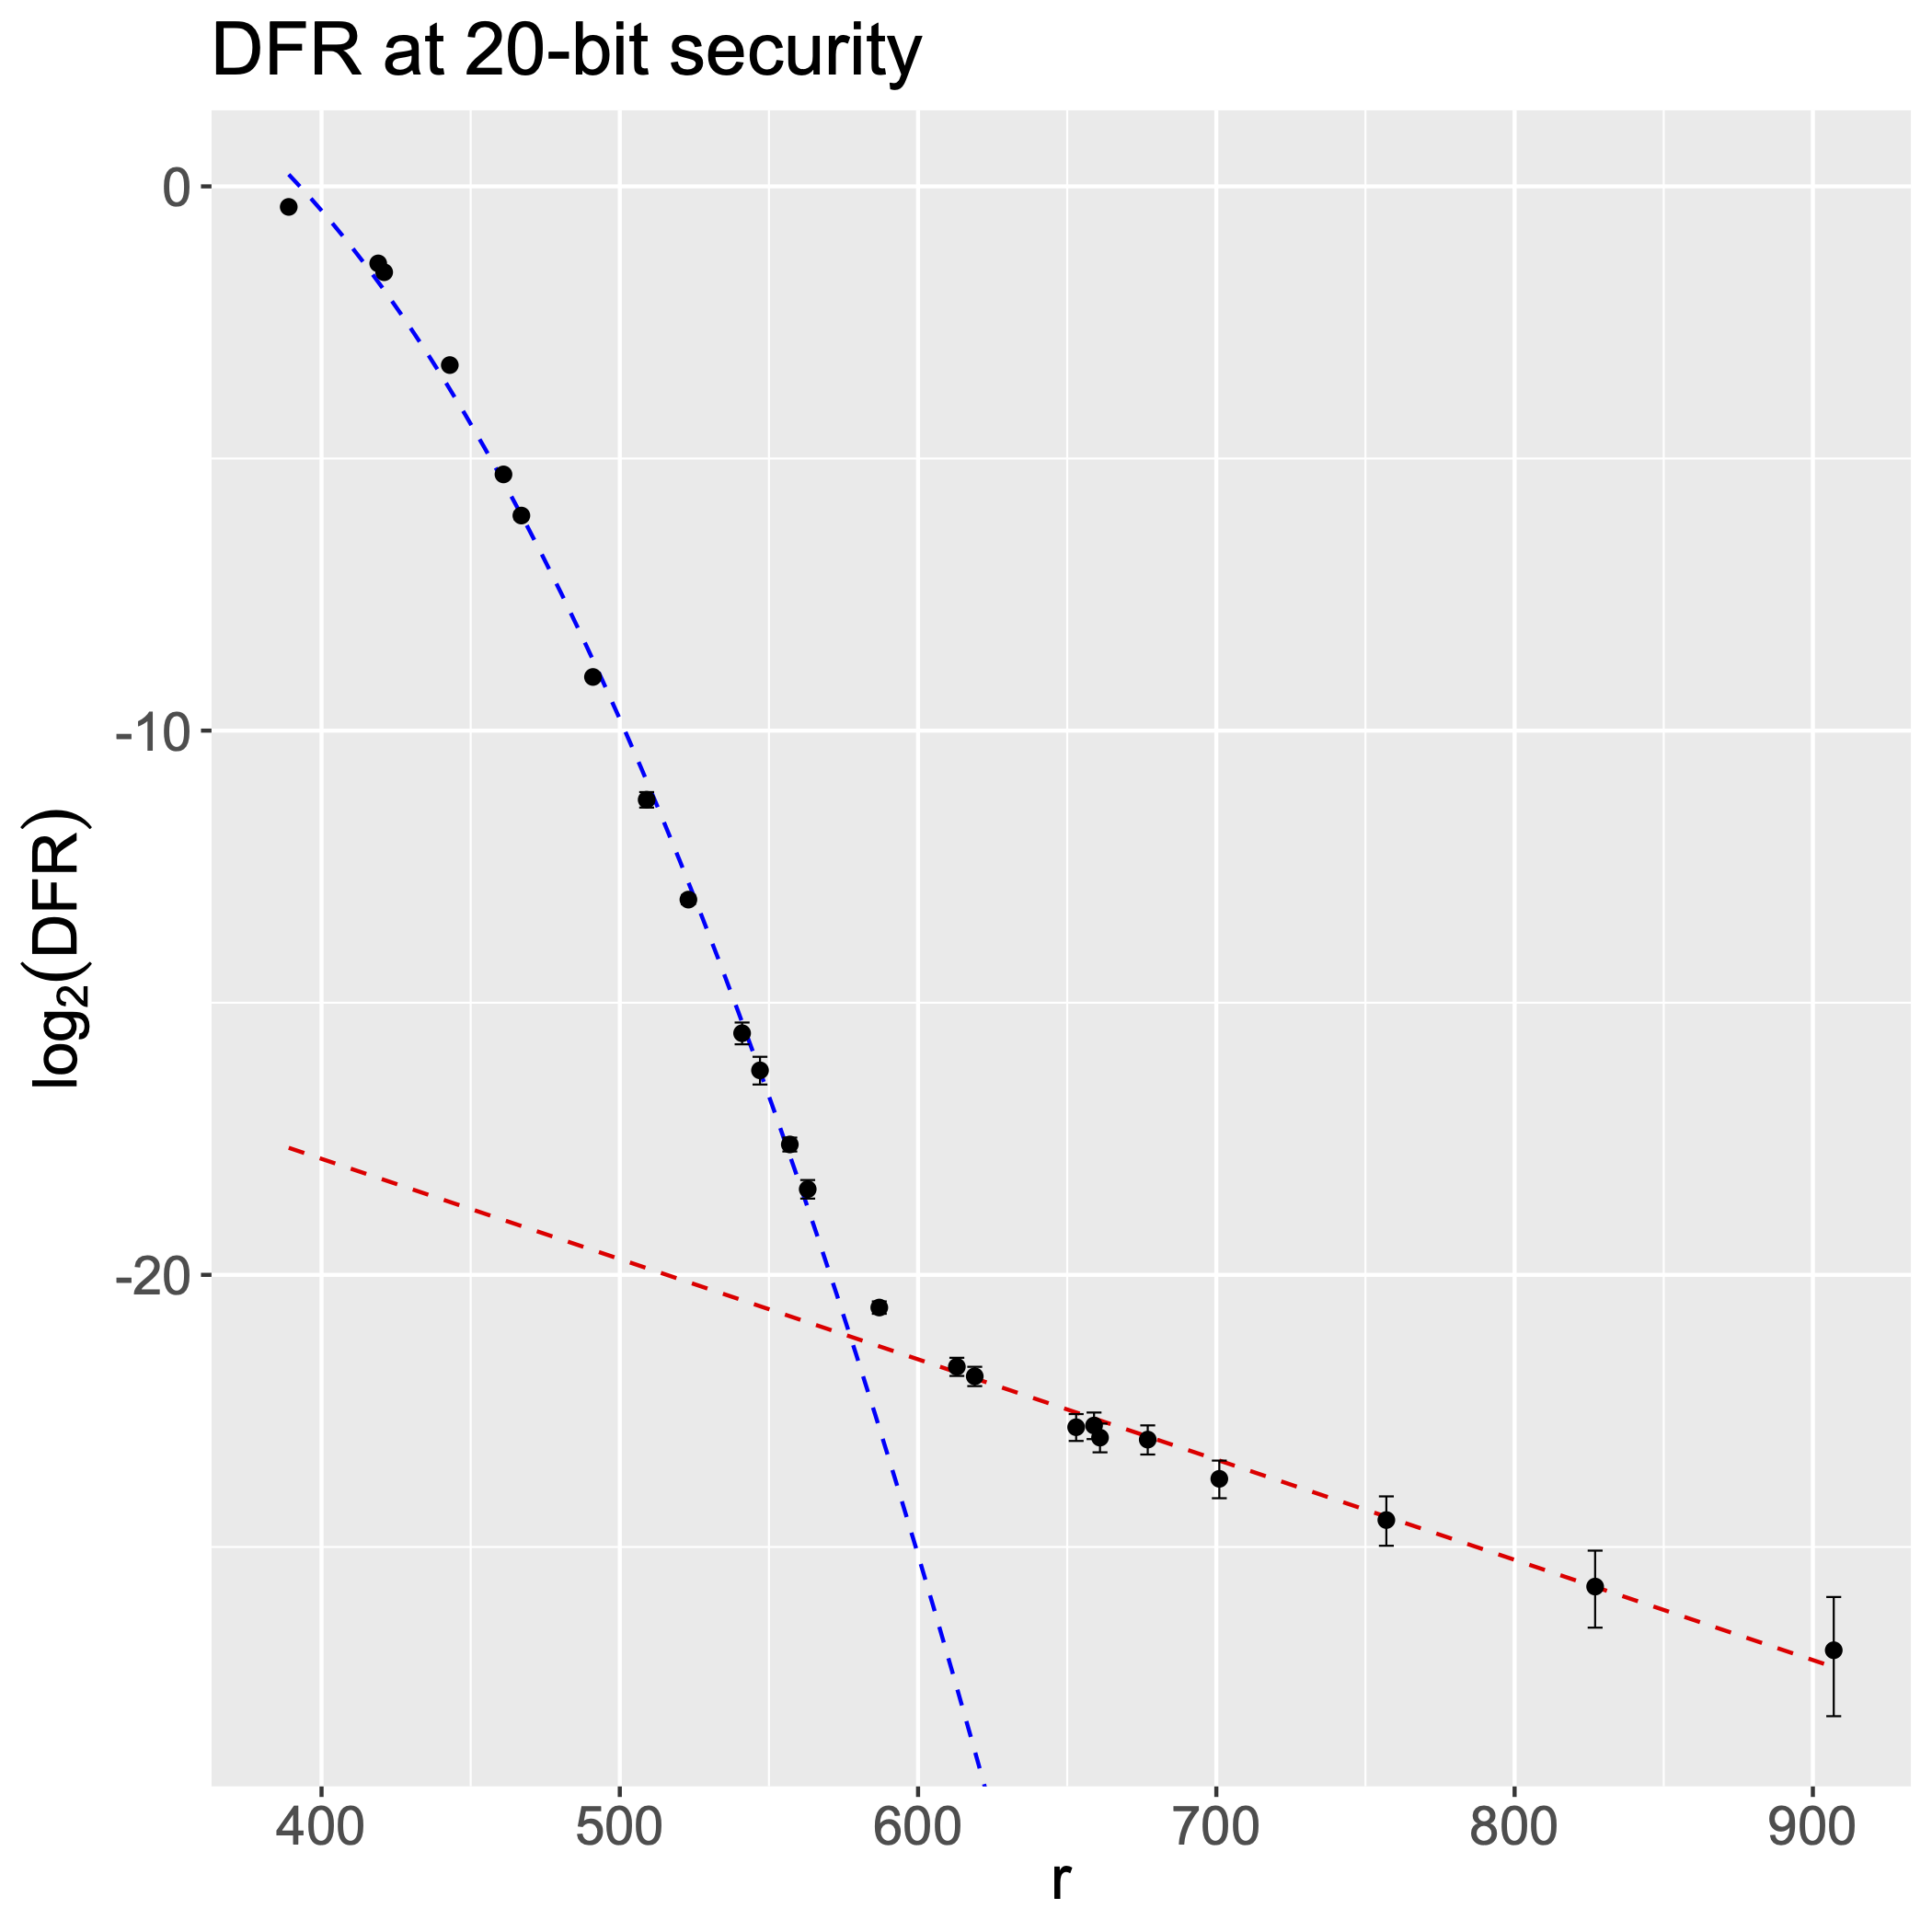
\includegraphics[width=0.49\textwidth]{2_bike/DFR-plot-T3.png}
    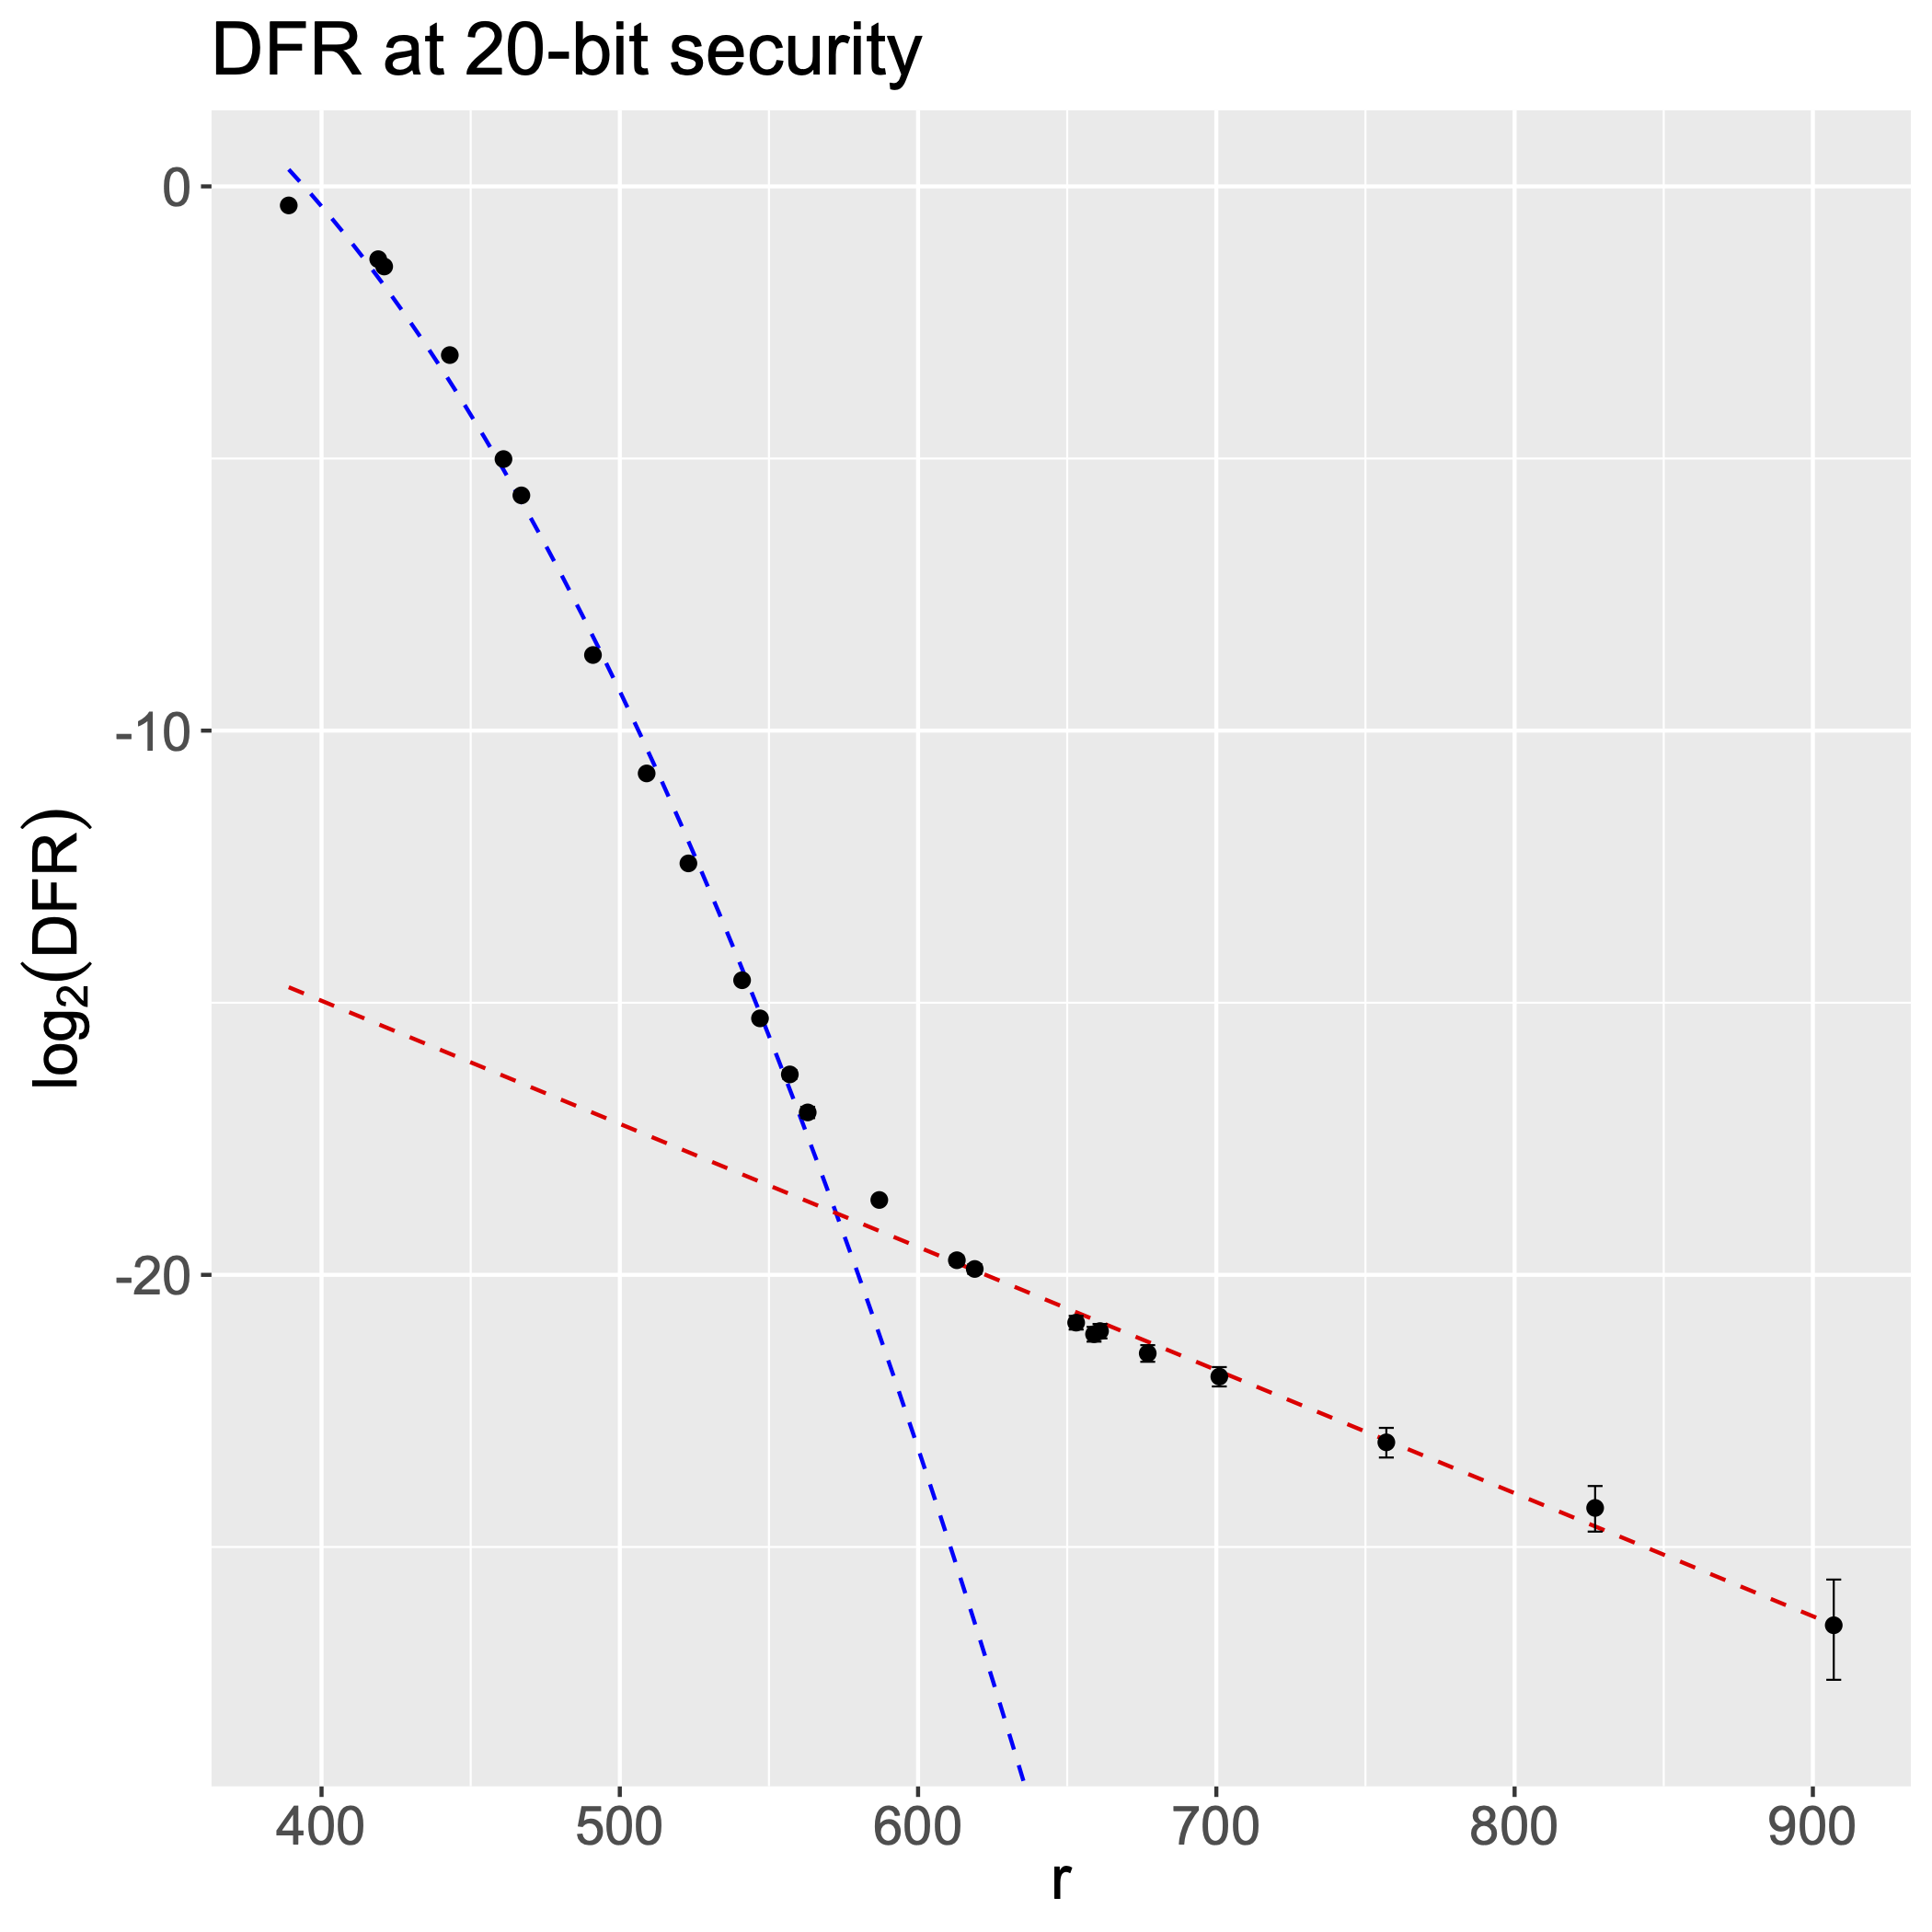
\includegraphics[width=0.49\textwidth]{2_bike/DFR-plot-random.png}
  \end{center}
  \caption{Semi-log plot of decoding failure rates for non-weak keys ($T = 3$, left) and for unfiltered random keys (right), with a 95\% confidence interval for each $r$. There is a quadratic best fit (blue) in the waterfall region and a linear best fit (red) in the error floor region ($r \geq 587$).}
  \label{fig:DFR}
\end{figure}

\newpage

\begin{flushleft}
    \textbf{Table 6.1}: Decoding failure rates for $r$-values such that $389 \leq r \leq 827$, $r$ is prime, and $x^r - 1$ has only two irreducible factors modulo $2$. The data was computed using the parameters and methods described above.
    \end{flushleft}
\begin{table}[htb]
    \begin{center}
        \begin{tabular}{c|c|c|r}
            \;\;\;$r$\;\;\; & \;Decoding failures\;  & \;Decoding trials\;  & \;$\log_2(\mathrm{DFR})$ \\
            \hline
            389 & 7544 & $10^4$ & $-0.41$ \\
            419 & 3482 & $10^4$ & $-1.52$ \\
            421 & 3167 & $10^4$ & $-1.66$ \\
            443 & 9182 & $10^5$ & $-3.45$ \\
            461 & 2134 & $10^5$ & $-5.55$ \\
            467 & 1304 & $10^5$ & $-6.26$ \\
            491 & 1506 & $10^6$ & $-9.38$ \\
            509 & 322 & $10^6$ & $-11.60$ \\
            523 & 916 & $10^7$ & $-13.41$ \\
            541 & 169 & $10^7$ & $-15.85$ \\
            547 & 109 & $10^7$ & $-16.49$ \\
            557 & 382 & $10^8$ & $-18.00$ \\
            563 & 263 & $10^8$ & $-18.54$ \\
            587 & 557 & $10^9$ & $-20.78$ \\
            613 & 272 & $10^9$ & $-21.81$ \\
            619 & 300 & $10^9$ & $-21.67$ \\
            653 & 144 & $10^9$ & $-22.73$ \\
            659 & 157 & $10^9$ & $-22.60$ \\
            661 & 126 & $10^9$ & $-22.92$ \\
            677 & 102 & $10^9$ & $-23.22$ \\
            701 & 83 & $10^9$ & $-23.52$ \\
            757 & 31 & $10^9$ & $-24.94$ \\
            827 & 15 & $10^9$ & $-25.99$ \\
	    907 & 7 & $10^9$ & $-27.09$
        \end{tabular}
    \end{center}
    \label{table:DFR}
\end{table}
